\subsubsection{Lược đồ Usecase}
Đối tượng thao tác trên hệ thống gồm có: Nhân viên và quản trị viên.\par
Các chức năng được đặc tả trong sơ đồ Usecase như Hình \ref{usecase} dưới đây.
\newpage
\begin{figure}[h!]
    \begin{center}
        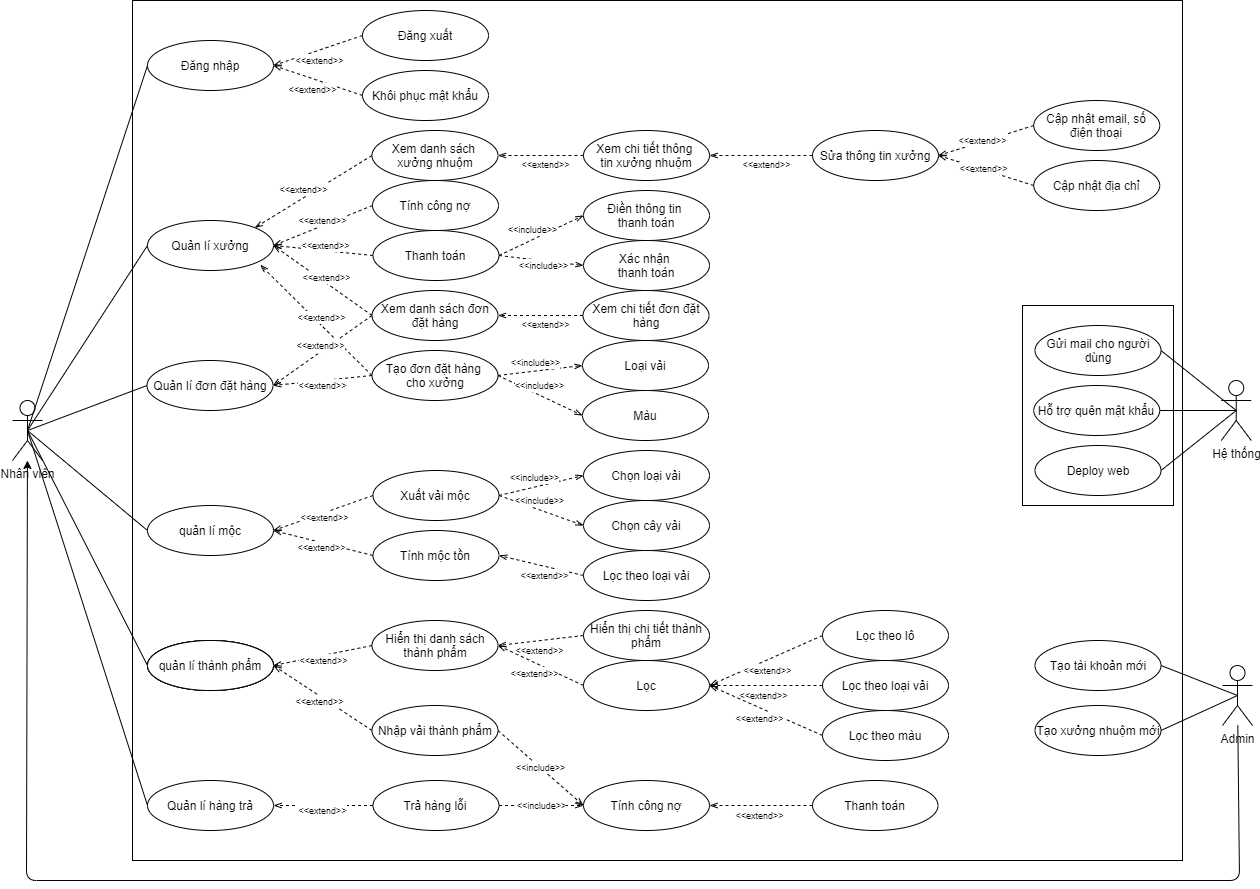
\includegraphics[width=16cm]{Image/General/Usecase.png}
        \caption{Usecase}
        \label{usecase}
    \end{center}
\end{figure}

\newpage
\subsubsection{Đặt tả Usecase}
\textbf{Đăng nhập}\par
\textbf{User story:} Là một người dùng của hệ thống, tôi muốn mình có thể đăng nhập vào để sử dụng hệ thống. Thông tin đăng nhập gồm có email và mật khẩu. Nếu tôi chưa đăng nhập, và cố gắng truy cập vào các trang của hệ thống, hệ thống sẽ chuyển hướng về trang đăng nhập. Nếu như quá 30 phút mà tôi không có hành động gì với hệ thống, thì phiên đăng nhập hết hạn và khi đó tôi sẽ phải đăng nhập lại. [\ref{bang1}]
\begin{table}[!htp]
    \centering
    \begin{tabular}{|m{3cm}|m{10cm}|}
    \hline 
        Use-case ID & 1\\ \hline
        Use-case name & Đăng nhập\\ \hline
        Actor & Nhân viên, quản trị viên.\\ \hline
        Description & Người dùng phải nhập tài khoản, mật khẩu để có thể sử dụng hệ thống.\\ \hline
        Preconditions & Người dùng đã đăng kí tài khoản và đang ở trang đăng nhập.\\ \hline
        Postconditions & Người dùng đã đăng nhập và có thể sử dụng hệ thống.\\ \hline
        Normal Flow & 
        1. Nhập tài khoản người dùng, hoặc email mà người dùng đã đăng kí cho tài khoản.\par
        2. Nhập mật khẩu.\par
        3. Bấm vào nút "Đăng nhập".
        \\ \hline
        Exception & 
        3a. Người dùng nhập tài khoản không chính xác.\par
        3b. Người dùng nhập mật khẩu không chính xác
        \\ \hline
        Alternative flow & Không có\\ 
    \hline 
    \end{tabular}
    \caption{Đăng nhập.}
    \label{bang1}
\end{table}

\textbf{Khôi phục mật khẩu}\par
\textbf{User story:} Là một người dùng của hệ thống, tôi muốn có thể khôi phục lại mật khẩu của mình trong trường hợp quên mật khẩu hoặc muốn cập nhật mật khẩu mới. Khi yêu cầu khôi phục mật khẩu, tôi sẽ phải cung cấp email của mình, sau đó một email sẽ được hệ thống gửi đến chưa một đường dẫn, khi nhấn vào đường dẫn tôi sẽ được chuyển đến trang nhập mật khẩu mới. Thời gian hết hạn của đường dẫn trong mail trên là 5 phút, khi đó tôi phải thực hiện lại yêu cầu khôi phục mật khẩu. [\ref{bang2}]
\begin{table}[!htp]
    \centering
    \begin{tabular}{|m{3cm}|m{10cm}|}
    \hline 
        Use-case ID & 2\\ \hline
        Use-case name & Khôi phục mật khẩu.\\ \hline
        Actor & Nhân viên, quản trị viên.\\ \hline
        Description & Người dùng quên mật khẩu tài khoản của mình thì vẫn có thể đặt lại mật khẩu mới qua xác thực email.\\ \hline
        Preconditions & Người dùng đã có tài khoản hệ thống.\\ \hline
        Postconditions & Người dùng đặt lại mật khẩu mới.\\ \hline
        Normal Flow & 
        1. Nhấn vào Quên mật khẩu trên trang đăng nhập.\par
        2. Nhập email đã đăng kí cho tài khoản.\par
        3. Hệ thống sẽ gửi email, trên email sẽ có đường link để đổi mật khẩu, nhấn vào link.\par
        4. Nhập mật khẩu mới.\par
        5. Nhấn xác nhận.
        \\ \hline
        Exception & 3a. Nếu không thấy email thì tài khoản này không tồn tại.\\ \hline
        Alternative flow & Không có.\\ 
    \hline 
    \end{tabular}
    \caption{Khôi phục mật khẩu.}
    \label{bang2}
\end{table}

\newpage
\textbf{Xem xưởng nhuộm}\par
\textbf{User story:} Là một người dùng của hệ thống, tôi có thể xem được danh sách các xưởng nhuộm đang làm việc với công ty mình. Thông tin mỗi xưởng nhuộm bao gồm Tên xưởng nhuộm, công nợ và số lượng vải mộc tồn kho ở xưởng. Khi nhấn vào một xưởng, tôi có thể xem thông tin chi tiết về xưởng nhuộm. Thông tin chi tiết của xưởng bao gồm: tên xưởng, địa chỉ, số điện thoại, email, công nợ, danh sách các đơn đặt hàng ở xưởng này. Ngoài ra, có thêm các nút chỉnh sửa thông tin, tạo đơn đặt hàng, tạo thanh toán và danh sách vải tồn, khi nhấn vào sẽ có các hành động tương ứng như tiêu đề. [\ref{bang3}]
\begin{table}[!htp]
    \centering
    \begin{tabular}{|m{3cm}|m{10cm}|}
    \hline 
        Use-case ID & 3\\ \hline
        Use-case name & Xem xưởng nhuộm.\\ \hline
        Actor & Nhân viên, quản trị viên.\\ \hline
        Description & Nhân viên có thể xem danh sách các xưởng nhuộm, bao gồm mã xưởng, tên xưởng, tổng công nợ và tổng độ dài mộc tồn. Nhân viên nhấn vào tên xưởng để xem thông tin chi tiết về xưởng.\\ \hline
        Preconditions & Người dùng đã đăng nhập vào hệ thống.\\ \hline
        Postconditions & Người dùng có thể xem các thông tin về xưởng nhuộm.\\ \hline
        Normal Flow & 
        1. Nhấn vào nút "Danh sách xưởng nhuộm" trên thanh menu, danh sách xưởng nhuộm xuất hiện.\par
        2. Nhấn vào tiêu đề trên mỗi cột để sắp xếp.\par
        3. Sử dụng bộ lọc để lọc thông tin.\par
        4. Nhấn vào xưởng nhuộm trong danh sách để chuyển sang trang Chi tiết xưởng nhuộm.\par
        \\ \hline
        Exception & Không có.\\ \hline
        Alternative flow & 
        Không có. \par
        \\ 
    \hline 
    \end{tabular}
    \caption{Xem xưởng nhuộm.}
    \label{bang3}
\end{table}

\newpage
\textbf{Chỉnh sửa thông tin xưởng nhuộm.}\par
\textbf{User story:} Là người dùng của hệ thống, tôi có thể chỉnh sửa các thông tin cơ bản của một xưởng nhuộm. Khi nhấn vào nút chỉnh sửa thông tin trong trang chi tiết xưởng nhuộm, tôi có thể sửa địa chỉ, số điện thoại và email của xưởng này. Sau khi cập nhật xong, tôi sẽ thấy thông tin mới trong trang chi tiết xưởng nhuộm. [\ref{bang4}]
\begin{table}[!htp]
    \centering
    \begin{tabular}{|m{3cm}|m{10cm}|}
    \hline 
        Use-case ID & 4\\ \hline
        Use-case name & Chỉnh sửa thông tin xưởng nhuộm.\\ \hline
        Actor & Nhân viên, quản trị viên.\\ \hline
        Description & Người dùng có thể chỉnh sửa một số thông tin cơ bản về xưởng nhuộm như địa chỉ, số điện thoại và email.\\ \hline
        Preconditions & Người dùng đã đăng nhập vào hệ thống.\\ \hline
        Postconditions & Thông tin về xưởng nhuộm sẽ được chỉnh sửa\\ \hline
        Normal Flow & 
        1. Trên trang thông tin chi tiết của xưởng, nhấm vào nút "Chỉnh sửa thông tin".\par
        2. Nhập địa chỉ, số điện thoại và email cần sửa.\par
        3. Nhấn nút "Lưu".
        \\ \hline
        Exception & 
        2a. Hệ thống sẽ hiển thị thông tin hiện tại của xưởng, người dùng chỉ cần chỉnh sửa thông tin nào cần thay đổi.
        2b. Người dùng nhập số điện thoại không đúng độ dài hoặc email sai định dạng, hệ thống sẽ báo lỗi.
        \\ \hline
        Alternative flow & 
        3a. Nhấn nút "Hủy bỏ" để hủy chỉnh sửa.
        \\ 
    \hline 
    \end{tabular}
    \caption{Chỉnh sửa thông tin xưởng nhuộm.}
    \label{bang4}
\end{table}

\newpage
\textbf{Thanh toán}\par
\textbf{User story:} Là người dùng của hệ thống, tôi có thể tạo hóa đơn thanh toán công nợ cho một xưởng nhuộm. Khi nhấn vào nút Tạo thanh toán trong trang chi tiết xưởng nhuộm, hoặc nhấn vào Tạo hóa đơn ở menu, tôi sẽ được chuyển qua trang tạo hóa đơn thanh toán.Ở đây, tôi nhập các thông tin gồm xưởng nhuộm, phương thức thanh toán, ngân hàng (nếu có), tổng số tiền, và nhân viên xác nhận thanh toán ở xưởng nhuộm. [\ref{bang5}]
\begin{table}[!htp]
    \centering
    \begin{tabular}{|m{3cm}|m{10cm}|}
    \hline 
        Use-case ID & 5\\ \hline
        Use-case name & Thanh toán\\ \hline
        Actor & Nhân viên, quản trị viên.\\ \hline
        Description & Người dùng có thể thanh toán tiền cho xưởng nhuộm.\\ \hline
        Preconditions & Người dùng đã đăng nhập vào hệ thống.\\ \hline
        Postconditions & Xưởng nhuộm được thanh toán.\\ \hline
        Normal Flow & 
        1. Trong trang chi tiết của xưởng nhuộm, nhấn vào nút "Tạo thanh toán", màn hình Tạo thanh toán xuất hiện.\par
        2. Chọn xưởng nhuộm, phương thức thanh toán, ngân hàng hoặc tên người nhận\par
        3. Nhập số tiền cần thanh toán\par
        4. Nhập tên nhân viên nhận.\par
        5. Nhấn nút "Tạo".
        \\ \hline
        Exception & 
        3a. Nhập số tiền thanh toán lớn hơn công nợ của xưởng, hệ thống sẽ báo lỗi.
        \\ \hline
        Alternative flow & 
        1a. Nhấn nút "Danh sách công nợ" trên thanh menu, danh sách công nợ xuất hiện, sau đó nhấn vào nút "Thanh toán" của xưởng cụ thể.\par
        4a. Nhất nút "Hủy bỏ" để hủy thanh toán.
        \\ 
    \hline 
    \end{tabular}
    \caption{Thanh toán cho xưởng nhuộm.}
    \label{bang5}
\end{table}

\newpage
\textbf{Xem đơn đặt hàng}\par
\textbf{User story:} [\ref{bang6}]
\begin{table}[!htp]
    \centering
    \begin{tabular}{|m{3cm}|m{10cm}|}
    \hline 
        Use-case ID & 6\\ \hline
        Use-case name & Xem đơn đặt hàng.\\ \hline
        Actor & Nhân viên, quản trị viên.\\ \hline
        Description & Nhân viên có thể xem danh sách các đơn đặt hàng, bao gồm mã đơn, tên xưởng, ngày đặt, loại vải, màu, độ dài đặt, đã nhận, trạng thái. Nhân viên nhấn đơn đặt hàng để xem thông tin chi tiết về đơn.\\ \hline
        Preconditions & Người dùng đã đăng nhập vào hệ thống.\\ \hline
        Postconditions & Người dùng có thể xem các thông tin về đơn đặt hàng.\\ \hline
        Normal Flow & 
        1. Nhấn vào nút "Đơn đặt hàng" trên thanh menu, danh sách đơn đặt hàng xuất hiện.\par
        2. Nhấn vào tiêu đề trên mỗi cột để sắp xếp.\par
        3. Sử dụng bộ lọc để lọc thông tin.\par
        3. Nhấn vào mã đơn để chuyển tới màn hình chi tiết của đơn đặt hàng.
        \\ \hline
        Exception & Không có.\\ \hline
        Alternative flow & 
        3a. Nhấn vào mã đơn trong danh sách đơn đặt hàng của trang thông tin chi tiết về xưởng để chuyển tới màn hình chi tiết của đơn đặt hàng.
        \\ 
    \hline 
    \end{tabular}
    \caption{Xem đơn đặt hàng.}
    \label{bang6}
\end{table}

\newpage
\textbf{Tạo đơn đặt hàng}
\textbf{User story:} [\ref{bang5}]
\begin{table}[!htp]
    \centering
    \begin{tabular}{|m{3cm}|m{10cm}|}
    \hline 
        Use-case ID & 7\\ \hline
        Use-case name & Tạo đơn đặt hàng.\\ \hline
        Actor & Nhân viên, quản trị viên.\\ \hline
        Description & Người dùng có thể tạo đơn đặt hàng nhuộm cho xưởng nhuộm.\\ \hline
        Preconditions & Người dùng đã đăng nhập vào hệ thống.\\ \hline
        Postconditions & Đơn đặt hàng mới được tạo\\ \hline
        Normal Flow & 
        1. Nhấn vào nút "Tạo đơn" trên thanh menu, màn hình tạo đơn đặt hàng sẽ xuất hiện.\par
        2. Chọn xưởng nhuộm, loại vải, màu.\par
        3. Nhập độ dài vải cần đặt.\par
        4. Nhấn nút "Tạo".
        \\ \hline
        Exception & \\ \hline
        Alternative flow & 
        1a. Nhấn vào nút "Tạo đơn đặt hàng" trên trang chi tiết của xưởng nhuộm.\par
        4a. Nhấn nút "Hủy bỏ" để hủy tạo đơn đặt hàng.
        \\ 
    \hline 
    \end{tabular}
    \caption{Tạo đơn đặt hàng.}
    \label{bang7}
\end{table}

\textbf{Xem vải mộc}
\textbf{User story:} [\ref{bang5}]
\begin{table}[!htp]
    \centering
    \begin{tabular}{|m{3cm}|m{10cm}|}
    \hline 
        Use-case ID & 8\\ \hline
        Use-case name & Xem vải mộc.\\ \hline
        Actor & Nhân viên, quản trị viên.\\ \hline
        Description & Người dùng có thể xem số lượng vải mộc tồn trong kho và mộc tồn tại xưởng. Mộc tồn được phân loại theo loại vải.\\ \hline
        Preconditions & Người dùng đã đăng nhập vào hệ thống.\\ \hline
        Postconditions & Người dùng có thể xem các thông tin về vải mộc tồn.\\ \hline
        Normal Flow & 
        1. Nhấn vào nút "Danh sách vải tồn" trên thanh menu, màn hình danh sách vải mộc xuất hiện.\par
        2. Xem vải mộc tại kho, chọn "Kho". Thống kê theo loại vải.\par
        3. Xem vải mộc tại xưởng, chọn "Xưởng". Thống kê theo xưởng và loại vải.
        \\ \hline
        Exception & Không có.\\ \hline
        Alternative flow & Không có.\\ 
    \hline 
    \end{tabular}
    \caption{Xem vải mộc.}
    \label{bang8}
\end{table}

\newpage
\textbf{Tạo phiếu xuất vải mộc}
\textbf{User story:} [\ref{bang5}]
\begin{table}[!htp]
    \centering
    \begin{tabular}{|m{3cm}|m{10cm}|}
    \hline 
        Use-case ID & 9\\ \hline
        Use-case name & Tạo phiếu xuất vải mộc\\ \hline
        Actor & Nhân viên, quản trị viên.\\ \hline
        Description & Người dùng tạo phiếu xuất vải mộc cho xưởng nhuộm, phiếu xuất gồm nhiều cây vải có thể nhiều thuộc loại vải khác nhau.\\ \hline
        Preconditions & Người dùng đã đăng nhập vào hệ thống.
        \\ \hline
        Postconditions & Xuất vải mộc cho xưởng nhuộm.\\ \hline
        Normal Flow & 
        1. Nhấn nút "Tạo phiếu xuất" trên thanh menu, trang tạo phiếu xuất vải mộc xuất hiện.\par
        2. Chọn xưởng nhuộm cần xuất.\par
        3. Nhập mã của từng cây vải, sau đó nhấn nút "Thêm", cây vải sẽ được thêm vào danh sách hiển thị ra màn hình.\par
        4. Nhấn nút "Tạo".
        \\ \hline
        Exception & Không có.
        \\ \hline
        Alternative flow & 
        4a. Có thể nhấn kí tự xóa để xóa cây vải ra khỏi danh sách nếu không muốn thêm vào phiếu xuất.\par
        4b. Nhấn nút "Hủy bỏ" để hủy phiếu xuất.
        \\ 
    \hline 
    \end{tabular}
    \caption{Tạo phiếu xuất vải mộc cho xưởng.}
    \label{bang9}
\end{table}

\textbf{Xem vải thành phẩm}
\textbf{User story:} [\ref{bang5}]
\begin{table}[!htp]
    \centering
    \begin{tabular}{|m{3cm}|m{10cm}|}
    \hline 
        Use-case ID & 10\\ \hline
        Use-case name & Xem vải thành phẩm.\\ \hline
        Actor & Nhân viên, quản trị viên.\\ \hline
        Description & Người dùng có thế xem danh sách các phiếu nhập vải thành phẩm từ xưởng, bao gồm mã phiếu, tổng thành phẩm, loại vải, màu, ngày nhộm.\\ \hline
        Preconditions & Người dùng đã đăng nhập vào hệ thống.\\ \hline
        Postconditions & Người dùng có thể xem thông tin về lô nhuộm và các cây vải thành phẩm trong lô.\\ \hline
        Normal Flow & 
        1. Nhấn vào nút "Danh sách phiếu nhập" trên thanh menu, trang danh sách phiếu nhập sẽ xuất hiện.\par
        2. Nhấn vào tiêu đề trên mỗi cột để sắp xếp.\par
        3. Sử dụng bộ lọc để lọc thông tin.
        \\ \hline
        Exception & Không có.\\ \hline
        Alternative flow & Không có.\\ 
    \hline 
    \end{tabular}
    \caption{Xem vải thành phẩm.}
    \label{bang10}
\end{table}

\newpage
\textbf{Tạo phiếu nhập vải thành phẩm}
\textbf{User story:} [\ref{bang5}]
\begin{table}[!htp]
    \centering
    \begin{tabular}{|m{3cm}|m{10cm}|}
    \hline 
        Use-case ID & 12\\ \hline
        Use-case name & Tạo phiếu nhập vải thành phẩm.\\ \hline
        Actor & Nhân viên, quản trị viên.\\ \hline
        Description & Người dùng sẽ tạo phiếu nhập vải thành phẩm từ xưởng nhuộm về kho. Mỗi phiếu nhập sẽ bao gồm nhiều cây vải thành phẩm.\\ \hline
        Preconditions & Người dùng đã đăng nhập vào hệ thống \\ \hline
        Postconditions & Phiếu nhập vải thành phẩm sẽ được tạo.\\ \hline
        Normal Flow & 
        1. Nhấn vào nút "Tạo phiếu nhập" trên thanh menu, trang tạo phiếu nhập sẽ xuất hiện.\par
        2. Nhập xưởng nhuộm, loại vải, màu cho lô nhuộm.\par
        3. Nhập mã đơn đặt hàng tương ứng.\par
        4. Nhấn nút "Tiếp theo".\par
        5. Nhập tên người giao hàng.\par
        6.  Nhập lần lượt mã cây vải và độ dài thành phẩm, sau đó nhấn nút "Thêm" để thêm cây vải vào lô nhuộm, danh sách cây vải của lô được hiển thị ra màn hình.\par
        4. Kiểm tra thông tin, nhấn nút "Tạo phiếu" để hoàn thành.
        \\ \hline
        Exception & Không có.
        \\ \hline
        Alternative flow & 
        6a. Nhấn vào kí tự xóa để xóa cây vải nêu không muốn thêm vào lô nhuộm nữa.
        \\ 
    \hline 
    \end{tabular}
    \caption{Tạo phiếu nhập vải thành phẩm từ xưởng nhuộm.}
    \label{bang11}
\end{table}

\textbf{Xem hàng trả}
\textbf{User story:} [\ref{bang5}]
\begin{table}[!htp]
    \centering
    \begin{tabular}{|m{3cm}|m{10cm}|}
    \hline 
        Use-case ID & 12\\ \hline
        Use-case name & Xem hàng trả\\ \hline
        Actor & Nhân viên, quản trị viên.\\ \hline
        Description & Người dùng có thể xem danh sách phiếu hàng trả. Mỗi phiếu hàng trả có thể có nhiều hàng trả. Người dùng có thể xem thông tin chi tiết của phiếu hàng trả bằng, bao gồm danh sách hàng trả của phiếu.\\ \hline
        Preconditions & Người dùng đã đăng nhập vào hệ thống.\\ \hline
        Postconditions & Người dùng xem được thông tin của phiếu hàng trả và danh sách hàng trả của phiếu hàng trả.\\ \hline
        Normal Flow & 
        1. Nhấn vào nút "Danh sách hàng trả" trên thanh menu, trang danh sách hàng trả xuất hiện.\par
        2. Nhấn vào mã phiếu để chuyển sang trang chi tiết về phiếu hàng trả.
        \\ \hline
        Exception & Không có\\ \hline
        Alternative flow & Không có\\ 
    \hline 
    \end{tabular}
    \caption{Xem hàng trả.}
    \label{bang12}
\end{table}

\newpage
\textbf{Tạo phiếu hàng trả}
\textbf{User story:} [\ref{bang5}]
\begin{table}[!htp]
    \centering
    \begin{tabular}{|m{3cm}|m{10cm}|}
    \hline 
        Use-case ID & 13\\ \hline
        Use-case name & Tạo phiếu hàng trả\\ \hline
        Actor & Nhân viên, quản trị viên.\\ \hline
        Description & Người dùng có thể tạo phiếu hàng trả, sau đó hàng trả sẽ lần lượt được thêm vào phiếu hàng trả.\\ \hline
        Preconditions & Người dùng đã đăng nhập vào hệ thống.\\ \hline
        Postconditions & Phiếu hàng trả và hàng trả được tạo.\\ \hline
        Normal Flow & 
        1. Nhấn vào nút "Tạo phiếu hàng trả" trên thanh menu.\par 
        2. Nhập tên người nhận hàng trả.\par
        3. Chọn xưởng nhuộm.\par 
        4. Nhập mã cây vải, độ dài trả, lí do trả.\par
        5. Nhấn nút "Tạo".
        \\ \hline
        Exception & Không có.
        \\ \hline
        Alternative flow & 
        5a. Nhấn nút "Hủy bỏ" để hủy phiếu hàng trả.
        \\ 
    \hline 
    \end{tabular}
    \caption{Tạo phiếu hàng trả}
    \label{bang13}
\end{table}

\textbf{Dashboard}
\textbf{User story:} [\ref{bang5}]
\begin{table}[!htp]
    \centering
    \begin{tabular}{|m{3cm}|m{10cm}|}
    \hline 
        Use-case ID & 14\\ \hline
        Use-case name & Dashboard\\ \hline
        Actor & Nhân viên, quản trị viên.\\ \hline
        Description & Người dùng có thể xem các thông tin thống kê.\\ \hline
        Preconditions & Người dùng đã đăng nhập vào hệ thống.\\ \hline
        Postconditions & Người dùng xem các thông tin thống kê.\\ \hline
        Normal Flow & 
        1. Thống kê sản lượng trong năm gần đây của từng xưởng nhuộm.\par
        2. Thống kê vải thành phẩm theo xưởng và Thống kê vải thành phẩm theo loại vải.\par
        3. Danh sách phiếu nhập gần đây.\par
        4. Danh sách phiếu xuất gần đây.
        \\ \hline
        Exception & Khống có.\\ \hline
        Alternative flow & Không có.\\ 
    \hline 
    \end{tabular}
    \caption{Dashboard}
    \label{bang14}
\end{table}

\newpage
\textbf{Tạo nhân viên mới}
\textbf{User story:} [\ref{bang5}]
\begin{table}[!htp]
    \centering
    \begin{tabular}{|m{3cm}|m{10cm}|}
    \hline 
        Use-case ID & 15\\ \hline
        Use-case name & Tạo nhân viên mới\\ \hline
        Actor & Quản trị viên.\\ \hline
        Description & Quản trị viên có thể tạo nhân viên mới.\\ \hline
        Preconditions & Quản trị viên đã đăng nhập vào hệ thống.\\ \hline
        Postconditions & Nhân viên mới được tạo.\\ \hline
        Normal Flow & 
        1. Nhấn vào nút "Tạo nhân viên" trên thanh menu.\par 
        2. Nhập họ tên nhân viên mới.\par
        3. Nhập email.\par
        4. Nhập mật khẩu.\par
        5. Nhập giới tính.\par
        6. Nhấn nút "Tạo".
        \\ \hline
        Exception & Không có.
        \\ \hline
        Alternative flow & 
        6a. Nhấn nút "Hủy bỏ" để hủy tạo nhân viên.
        \\ 
    \hline 
    \end{tabular}
    \caption{Tạo nhân viên}
    \label{bang15}
\end{table}

\textbf{Tạo xưởng nhuộm mới}
\textbf{User story:} [\ref{bang5}]
\begin{table}[!htp]
    \centering
    \begin{tabular}{|m{3cm}|m{10cm}|}
    \hline 
        Use-case ID & 16\\ \hline
        Use-case name & Tạo xưởng nhuộm mới\\ \hline
        Actor & Quản trị viên.\\ \hline
        Description & Quản trị viên có thể tạo xưởng nhuộm mới.\\ \hline
        Preconditions & Quản trị viên đã đăng nhập vào hệ thống.\\ \hline
        Postconditions & Xưởng nhuộm mới được tạo.\\ \hline
        Normal Flow & 
        1. Nhấn vào nút "Tạo xưởng nhuộm" trên thanh menu.\par 
        2. Nhập tên xưởng.\par
        3. Nhập địa chỉ.\par
        4. Nhập số điện thoại.\par
        5. Nhập email.\par
        6. Nhấn nút "Tạo".
        \\ \hline
        Exception & Không có.
        \\ \hline
        Alternative flow & 
        6a. Nhấn nút "Hủy bỏ" để hủy tạo xưởng nhuộm.
        \\ 
    \hline 
    \end{tabular}
    \caption{Tạo xưởng nhuộm}
    \label{bang16}
\end{table}

% \textbf{User story:} [\ref{bang5}]
% \begin{table}[!htp]
%     \centering
%     \begin{tabular}{|m{3cm}|m{10cm}|}
%     \hline 
%         Use-case ID & 1\\ \hline
%         Use-case name & \\ \hline
%         Actor & \\ \hline
%         Description & \\ \hline
%         Preconditions & \\ \hline
%         Postconditions & \\ \hline
%         Normal Flow & \\ \hline
%         Exception & \\ \hline
%         Alternative flow & \\ 
%     \hline 
%     \end{tabular}
%     \caption{Đăng nhập}
%     \label{bang1}
% \end{table}